\documentclass{article}
\usepackage{fancyhdr}
\usepackage{ctex}
\usepackage{listings}
\usepackage[a4paper, body={18cm,22cm}]{geometry}
\usepackage{amsmath,amssymb,amstext,wasysym,enumerate,graphicx}
\usepackage{float,abstract,booktabs,indentfirst,amsmath}
\usepackage{multirow}
\usepackage{enumitem}
\usepackage{listings}
\usepackage{xcolor}
\usepackage{tabularx}
\usepackage[most]{tcolorbox}
\usepackage{accsupp}
\usepackage[bottom]{footmisc}
\usepackage{subcaption}
\usepackage{longtable}
% \usepackage[backend=biber,style=numeric]{biblatex}
\usepackage[xetex]{hyperref}
\usetikzlibrary{arrows.meta}
\newcommand\emptyaccsupp[1]{\BeginAccSupp{ActualText={}}#1\EndAccSupp{}}
\setlength{\parindent}{2em}
\renewcommand\arraystretch{1.4}
\setmonofont{Fira Code}
\setCJKmonofont{黑体}
% \setmainfont{Times New Roman}
\hypersetup{CJKbookmarks=true,colorlinks=true,citecolor=blue,%
            linkcolor=blue,urlcolor=blue,bookmarksnumbered=true,%
            bookmarksopen=true,breaklinks=true}
\lstset{
    % language = C,
    xleftmargin = 3em,xrightmargin = 3em, aboveskip = 1em,
	backgroundcolor = \color{white}, % 背景色
	basicstyle = \small\ttfamily, % 基本样式 + 小号字体
	rulesepcolor= \color{gray}, % 代码块边框颜色
	breaklines = true, % 代码过长则换行
	numbers = left, % 行号在左侧显示
	numberstyle = \small\emptyaccsupp, % 行号字体
    numbersep = 14pt, 
    keywordstyle=\color{purple}\bfseries, % 关键字颜色
    commentstyle =\color{red}, % 注释颜色
    stringstyle = \color{red}, % 字符串颜色
    morekeywords={ASSERT, int64_t, uint32_t},
	frame = single, 
	showspaces = false, % 不显示空格
    showstringspaces = false,
	columns = fixed, % 字间距固定
    literate=
        {^-}{{{\color{black}\textbf{\color{red}-}}\colorbox{red!30}{\phantom{XX}}}}{1}
        {^+}{{{\color{black}\textbf{\color{green}+}}\colorbox{green!30}{\phantom{XX}}}}{1},
}

\raggedbottom

\title{\textbf{路径引导策略设计说明}}
\author{第七组 \\ 
李鹏达 10225101460 \\[-1em]
张耘彪 10225101437 \\[-1em]
武泽恺 10225101429
}
\date{}

\begin{document}
\maketitle

\section{背景介绍}

\linespread{1.5}

K{\small\MakeUppercase{ea}}当前实现了一种大模型引导的路径探索策略,主要负责在应用状态空间中遇到难以探索的UI状态时,利用大语言模型(LLM)生成输入事件以增强功能场景覆盖。该策略的设计旨在提高自动探索的效率和成功率,尤其是在面对复杂或动态变化的应用界面时。该策略的核心步骤是。首先,系统采用随机探索策略进行初步的UI状态遍历,并记录访问过的状态。当检测到当前状态与历史状态高度相似时,系统判定为陷入UI陷阱(即难以跳出的重复或无效状态)。此时,策略动态调用LLM,基于当前界面信息和可执行操作生成最优输入事件,以引导系统跳出UI陷阱。现有实验表明,该策略在一些应用场景中表现良好,能够有效地引导选择更优的操作序列,避免陷入死循环或无响应状态。

然而,在之前的探索中,我们发现该策略在处理UI陷阱时存在一定的局限性,在某些情况下,模型生成的操作序列可能无法有效跳出当前状态,导致陷入死循环或无响应状态。比如,我们在对\textit{Omninotes}进行测试时,发现软件中存在一个明显的UI陷阱,如图 \ref{fig:ui_trap_example1} 所示,该界面必须在填写表单后才能点击按钮进行跳转,而在随机探索的策略下,K{\small\MakeUppercase{ea}}会陷入死循环,无法有效地跳出该页面。我们尝试使用大模型生成操作序列,但发现生成的操作序列仍然无法有效地跳出该页面,导致陷入死循环。另外一个例子是,我们在对\textit{AnkiDroid}进行测试时,发现K{\small\MakeUppercase{ea}}会由于软件申请权限而跳转至一个权限申请页面,如图 \ref{fig:ui_trap_example2} 所示,在随机探索的策略下会陷入UI陷阱,然而,在原有的LLM探索策略下,我们发现大模型生成的操作序列并不能有效地跳出该页面。

经过分析,我们认为该问题主要源于以下几个方面:

\textbf{操作序列生成的准确性较低}:当前的操作序列生成依赖于当前界面上可提供的操作信息,然而,原有策略中提供的信息可能不足,且缺乏对界面结构的深入理解,导致生成的操作序列不够准确。比如,对于一个页面中的按钮,原有策略仅提供少量的文本信息,我们截取了 Prompt 切片如下:

\begin{lstlisting}[language=Python]
- a view with text "FOLDER" that can click (1);
- a view with text "CANCEL" that can click (2);
- a view with text "OK" that can click (3);
\end{lstlisting}

在这样的 Prompt 下,我们猜测大模型可能很难理解该页面的结构和功能,导致生成的操作序列不够准确。

\textbf{缺乏有效的错误处理机制}:在遇到无效操作或死循环时,现有大预言模型引导策略缺乏有效的错误处理机制,导致系统无法及时调整探索策略。比如,现有大预言模型引导策略仅考虑了当前事件的生成,而没有考虑到可能出现的错误情况,如操作失败等。这使得系统在遇到错误时无法及时调整策略,导致探索效率低下,重复执行无效操作。

因此,我们认为有必要对现有的路径引导策略进行改进,以提高其在UI陷阱中的表现。我们提出了一种新的路径引导策略,旨在通过引入更丰富的上下文信息和有效的错误处理机制,来提升操作序列生成的准确性和系统的鲁棒性。

\begin{figure*}[h]
    \begin{minipage}
        [t]{0.4\textwidth}
            \centering
            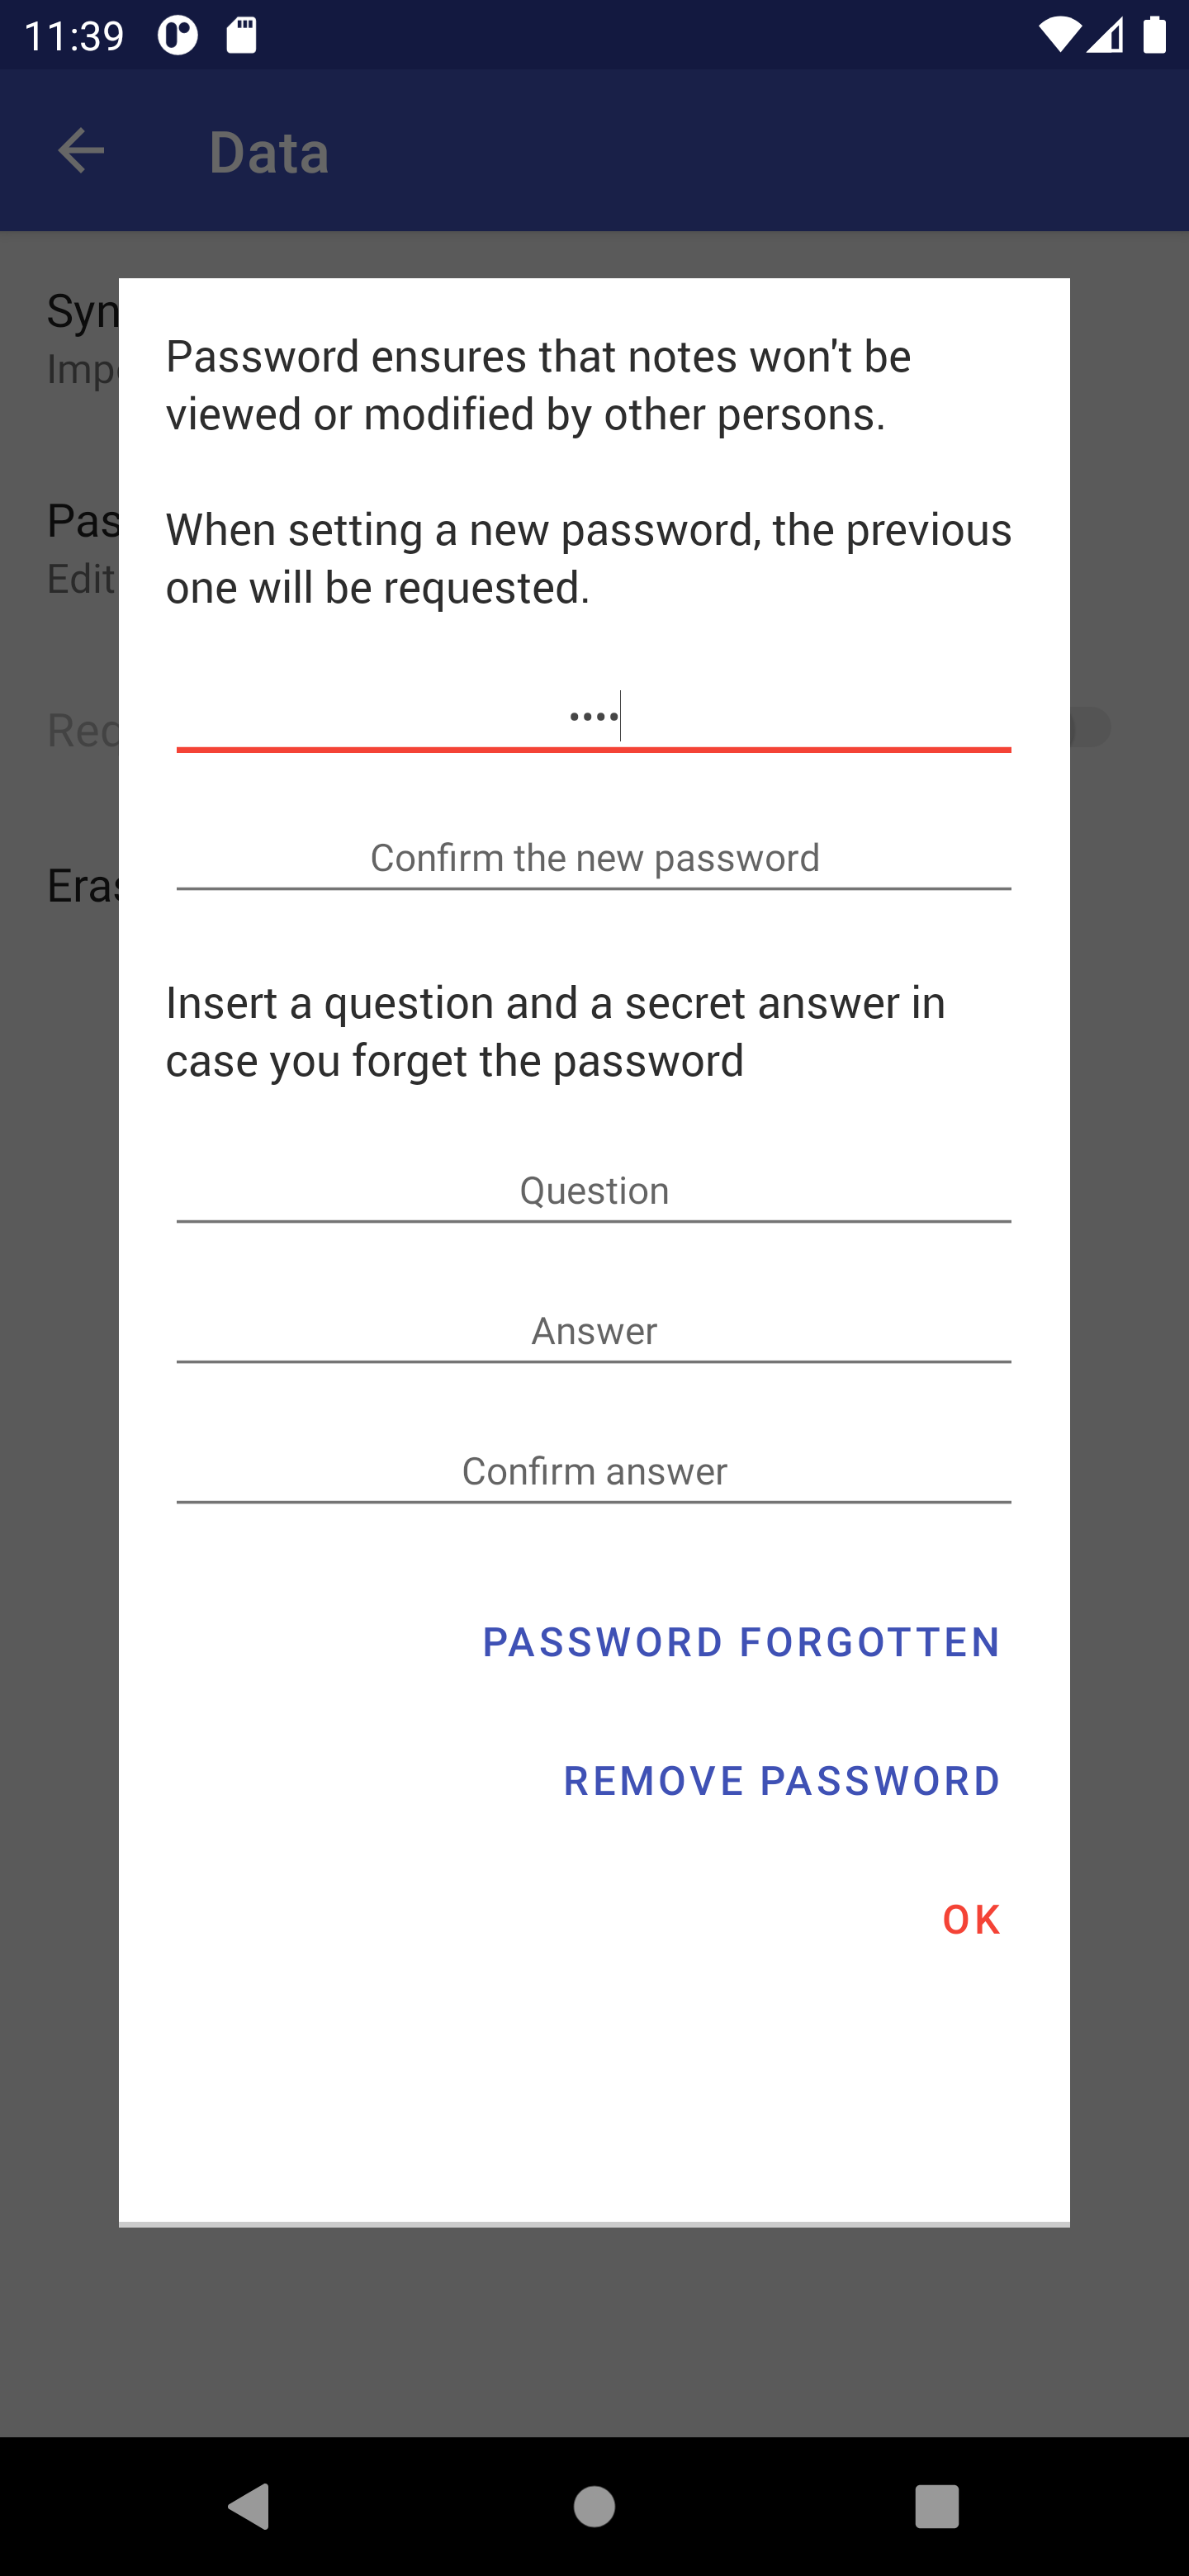
\includegraphics[width=0.8\textwidth]{1.png}
            \caption{Omninotes应用UI陷阱示例}
            \label{fig:ui_trap_example1}
        \end{minipage}
    \hfill
    \begin{minipage}
        [t]{0.4\textwidth}
            \centering
            
\includegraphics[width=0.8\textwidth]{2.png}
            \caption{AnkiDroid应用UI陷阱示例}
            \label{fig:ui_trap_example2}
        \end{minipage}
\end{figure*}

\section{大语言模型路径引导策略设计}

为了应对自动探索应用过程中可能遇到的UI陷阱(例如某些界面无响应、需特定操作才能离开、无效路径循环等),本系统引入了大语言模型(LLM)辅助的路径引导机制。具体设计流程如下:

\subsection{策略概述}
在探索过程中,若发现当前UI状态难以探索或无交互反馈,则通过LLM生成用户可能执行的操作序列,用于尝试跳出陷阱状态。这一策略的设计核心是将UI界面的结构(以XML表示)作为上下文输入,利用语言模型生成可能的用户意图与操作,并自动执行以引导状态转移。


\begin{figure}[H]
    \centering
    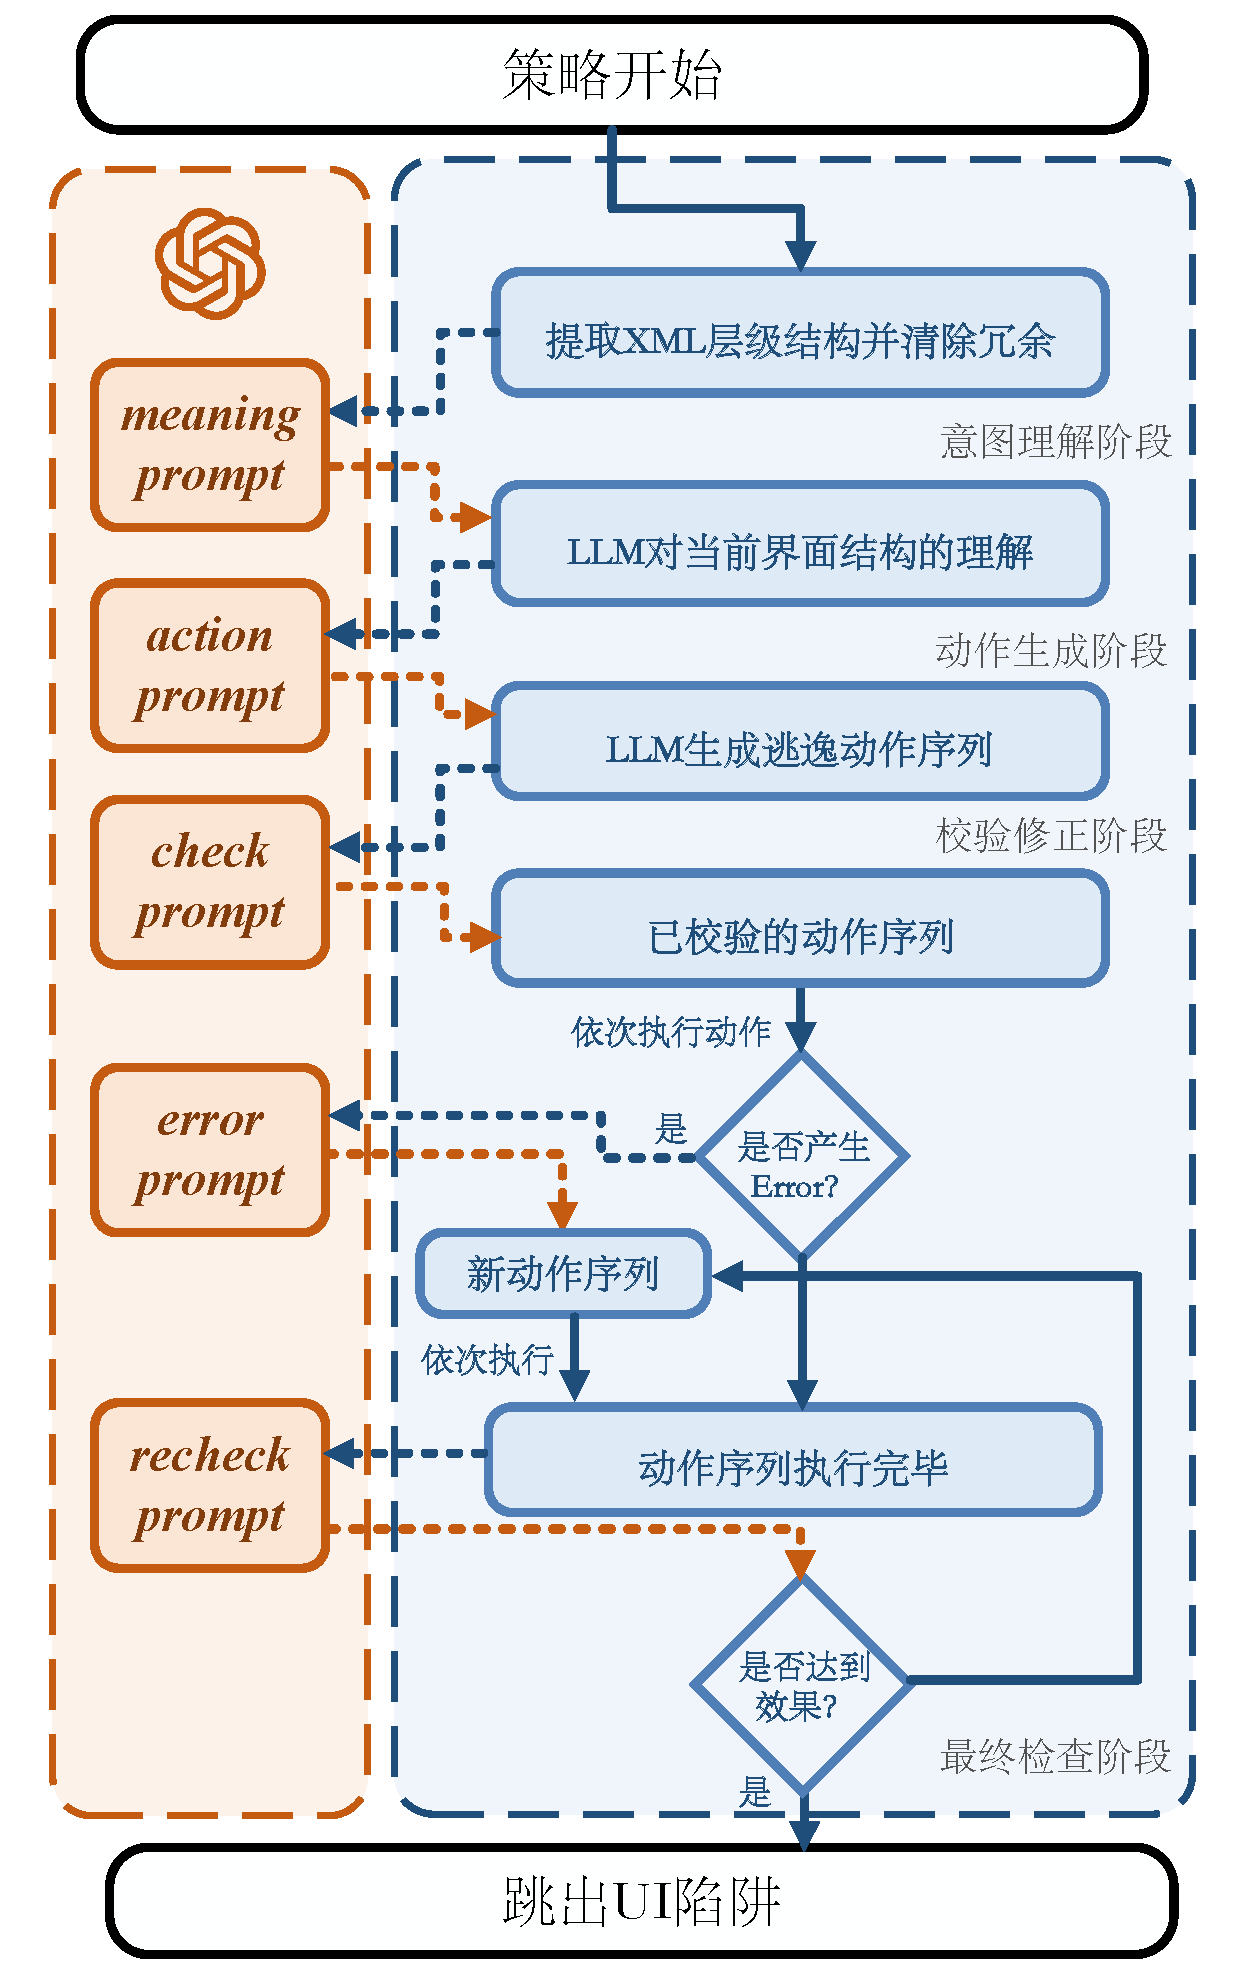
\includegraphics[width=0.5\textwidth]{3.png}
    \caption{示意图}
    \label{fig:strategy_overview}
\end{figure}

图 \ref{fig:strategy_overview} 展示了该策略的整体设计流程。

\subsection{四级提示工程}


我们考虑在进行提示词工程时,将一个问题拆解为多个步骤、逐渐引导提问,从而减少细节丢失,并模拟人类思维,优化大语言模型的效果。

具体来说,我们将提示工程分成四个阶段:意图理解阶段、动作生成阶段、校验修正阶段和最终检查阶段。每个阶段的设计旨在引导大语言模型更好地理解当前界面的结构和功能,逐步完成稳如,从而生成更准确的操作序列,并对结果进行自我检查和修正,减少出错。此外,我们还引入了错误处理机制,以确保在遇到无效操作时,系统能够及时调整探索策略。


\subsubsection{意图理解阶段} 

在这一阶段,我们将获取到的XML结构作为上下文输入到大语言模型中,要求其理解当前界面的意图和功能。

通过 \texttt{uiautomator2} 获取的XML结构内容比较复杂,含有大量无用和干扰信息,因此,我们首先对XML数据进行预处理。首先,我们去除了XML中系统状态栏的结构信息,以减少干扰。其次,我们删除了值为空字符串和 \texttt{false}的属性,以精简XML,减少无用信息。

我们设计了一个提示词 \texttt{meaning\_prompt()},用于引导模型生成对当前界面的描述。通过获取到模型对当前界面结构的理解,我们可以更好地引导模型生成后续的操作序列。
\begin{lstlisting}[language=Python]
prompt = f"""This is an XML representation of an Android application page:
{get_xml()}
Please describe the purpose of this page in the most concise language possible."""
\end{lstlisting}

\subsubsection{动作生成阶段} 

在这一阶段,我们根据之前的上下文信息,向大语言模型提出新的要求——要求其生成可能的用户操作序列。

我们设计了一个提示词 \texttt{action\_prompt()},用于引导模型生成可执行的操作序列。该提示词要求模型输出符合JSON格式的操作序列,并包含必要的属性信息。

在这个阶段,我们的方法与现有大语言模型引导策略中最大的区别是,现有的策略告诉大语言模型``你是一个自动测试专家'',而我们的方法告诉它\textbf{``你是用户''}。我们认为,在进行功能测试时,以用户的视角来理解界面和操作序列是非常重要的。用户在使用应用时,往往会根据界面的提示和功能进行操作。

此外,在此处,我们并不向大语言模型提及``UI陷阱'',而是将其视为一个普通的页面。因为我们发现,如果告诉大语言模型``这是一个UI陷阱'',它可能会更倾向于``逃避''和表现``无能为力'',而不是积极地寻找解决方案。我们希望它能够以用户的身份来理解界面,并生成相应的操作序列。

\begin{lstlisting}[language=Python]
prompt = f"""If you were the user, what would you do on this page?
Please provide an action or a sequence of actions in JSON format, for example:
[{{
    "action": "click",
    "selectors": {{"resourceId": "com.example:id/button1"}}
}},
{{
    "action": "input_text",
    "selectors": {{"resourceId": "com.example:id/input", "text": "password"}}
    "inputText": "123456"
}}]
Where:
- action can only be one of: click, long_click, input_text, press, swipe, scroll
- selector can only be one of: text, className, description, resourceId (must be in camelCase); choose the selector that uniquely identifies the element
- the selector's value and must be found in the provided XML
- inputText is the input text, applicable only when action is input_text
- pressKey can be "enter" and applicable only if action is "press"

Please combine multiple selectors to ensure uniquely locating an element.

Before outputting, check whether the value exists in the XML. If it does not exist, modify the action accordingly.

Return only the JSON-formatted action sequence, without explanations or code blocks."""
\end{lstlisting}

\subsubsection{校验修正阶段} 

在这一阶段,我们要求大语言模型进行自我检查,检查其生成的操作序列是否符合要求,以进一步提高操作序列的准确性。

我们设计了一个提示词 \texttt{check\_prompt()},用于引导模型检查生成的操作序列是否符合要求。通过这一阶段的校验,我们可以尽量保证生成的操作序列是可执行的,并且在LLM的经验判断下能够有效地跳出UI陷阱。


\begin{lstlisting}[language=Python]
prompt = """Please check whether the operation or sequence of operations you just generated meets the requirements:
- The selector must be found in the XML.
- The selector must uniquely identify the element.
- This sequence of operations must be executable on the current page.
If there are no issues, output it as is; otherwise, modify it accordingly."""
\end{lstlisting}

\subsubsection{最终校验阶段} 

在这一阶段之前,我们执行生成的操作序列,并尝试跳出UI陷阱。我们会在执行操作序列后,重新获取当前界面的XML结构,并要求大预言模型判断当前页面是否与执行操作前的状态相似。

我们设计了一个提示词 \texttt{recheck\_prompt()},用于引导模型判断当前页面是否与之前的状态相似。这一阶段的设计旨在检验生成的操作是否能够达成 ``跳出UI陷阱''的目的,如果不能跳出,我们再告诉大语言模型 ``逃离页面'',并要求其生成新的操作序列,以可能较为消极的方式来处理UI陷阱。

\begin{lstlisting}[language=Python]
prompt = """Please determine whether the current page is very very similar to the previously displayed XML page.
{get_xml()}
If it is very very similar, find a way to leave the page, output "YES", and then output the operation sequence according to the previous rules.
If it is not similar, output "NO"."""
\end{lstlisting}

\subsection{错误处理机制} 

在执行操作序列时,我们可能会遇到一些错误情况,例如元素不存在、操作失败等。为了应对这些错误情况,我们设计了一个错误处理机制。此外,我们还观察到,某些操作会导致当前页面发生变化,从而导致后续操作无法执行,引发上述的错误。

因此,我们在执行操作序列时,增加了一个错误处理机制。当我们发现错误时,将重新获取当前页面状态,并重新生成操作序列。我们设计了一个提示词 \texttt{error\_prompt()},用于引导模型修正错误。在这种情况下,我们仍然要保留之前的上下文信息,以便大语言模型能够意识到先前的操作,并在此基础上进行修正。

\begin{lstlisting}[language=Python]
prompt = f"""The event sequence you generated encountered an error because the corresponding element could not be found. This is the current XML representation of the application.
{get_xml()}
Correct this error. Output the operation sequence according to the previous rules."""
\end{lstlisting}

\section{实验}

为此,我们在不同的应用场景中进行了实验,测试了该策略在不同应用中的表现。由于时间有限,我们先进行了小规模的测试,我们选择了\textit{AnkiDroid}、\textit{Markor}和\textit{Omninotes}等应用进行测试,并将实验结果与现有的路径引导策略进行了对比分析。

\subsection{实验步骤}

首先,我们修改了 K{\small\MakeUppercase{ea}} 中对UI陷阱的检测策略,改为连续5次操作后,页面的相似度均超过87\%时,判定为UI陷阱。然后,我们在上述三款应用上运行了K{\small\MakeUppercase{ea}},并记录所找到的UI陷阱。为方便实验,我们将原有大语言模型引导策略代码抽取出来,并进行了适当的修改,以便于我们进行实验。我们将原有的路径引导策略称为 ``old'',而我们提出的路径引导策略称为 ``our''。在实验中,我们将 ``old'' 和 ``our'' 的结果进行了对比分析,并计算了通过率。

此外,我们还抽取了AURORA的分类器,以对这些找到的UI陷阱进行分类。以检查我们的方法是否适用于各类UI陷阱。我们将AURORA的分类结果称为 ``AURORA classify''。

\subsection{实验结果与分析}

\begin{longtable}[H]{lrrr}
        \toprule
        \textbf{Tarpit} & \textbf{old} & \textbf{our} & \textbf{AURORA classify} \\
        \midrule
        \endfirsthead
        \toprule
        \textbf{Tarpit} & \textbf{old} & \textbf{our} & \textbf{AURORA classify} \\
        \midrule
        \endhead
        $anki_0$ & -1 & 1 & 20 Web browser \\
        $anki_2$ & -1 & 1 & 16 Terms and conditions \\
        $anki_3$ & -1 & 1 & 11 Pop up menu \\
        $anki_4$ & 2 & 2 & 13 Search screen \\
        $anki_5$ & 1 & 1 & 13 Search screen \\
        $anki_6$ & 1 & 1 & 11 Pop up menu \\
        $anki_7$ & 1 & 2 & 11 Pop up menu \\
        $anki_8$ & 3 & 1 & 11 Pop up menu \\
        $anki_9$ & -1 & 4 & 4 Form screen \\
        $anki_{10}$ & 1 & 1 & 18 Type message \\
        $markor_0$ & -1 & -1 & 11 Pop up menu \\
        $markor_2$ & -1 & -1 & 6 List screen \\
        $markor_6$ & -1 & 2 & 11 Pop up menu \\
        $ominotes_0$ & -1 & 1 & 13 Search screen \\
        $ominotes_2$ & 2 & 2 & 6 List screen \\
        $ominotes_4$ & -1 & -1 & 6 List screen \\
        $ominotes_5$ & -1 & 1 & 6 List screen \\
        $ominotes_6$ & -1 & 2 & 6 List screen \\
        $ominotes_{19}$ & 2 & 1 & 6 List screen \\
        $ominotes_{23}$ & -1 & 1 & 18 Type message \\
        $ominotes_{25}$ & -1 & 1 & 16 Terms and conditions \\
        $ominotes_{26}$ & -1 & 1 & 11 Pop up menu \\
        $ominotes_{28}$ & 2 & 2 & 18 Type message \\
        $ominotes_{30}$ & 4 & 1 & 18 Type message \\
        \midrule
        $pass$ & 10 & 21 & \\
        $pass/total$ & 41.67\% & 87.5\% & \\
        $pass_1$ & 4 & 14 & \\
        $pass_1/total$ & 16.67\% & 58.33\% & \\
        \bottomrule
    \caption{实验结果}
    \label{tab:实验结果}
\end{longtable}

表 \ref{tab:实验结果} 展示了在不同的UI陷阱中,现有的路径引导策略和我们提出的路径引导策略在处理时的表现。其中,-1表示在5次尝试中未能跳出UI陷阱,其余数字表示需要跳出UI陷阱所尝试的次数。
$pass$ 表示成功跳出UI陷阱的数量,$pass/total$ 表示成功跳出UI陷阱的比例。$pass_1$ 在一次尝试中成功跳出UI陷阱的数量,$pass_1/total$ 表示一次尝试就成功跳出UI陷阱的比例。

实验数据表明,我们提出的路径引导策略在处理UI陷阱时,表现明显优于现有的路径引导策略。在所有的UI陷阱中,我们提出的路径引导策略成功跳出了21个UI陷阱,而现有的路径引导策略仅成功跳出了10个UI陷阱。且对于大多数的UI陷阱,我们的策略在1次尝试中成功跳出,而现有的引导策略往往要尝试多次或不能成功。

AURORA分类器的分类结果表明,我们的方法在处理不同类型的UI陷阱时,表现也较为稳定。我们的方法在处理 ``Web browser''、``Terms and conditions''、``Pop up menu''、``Search screen''、``List screen'' 和 ``Type message'' 等类型的UI陷阱时,均表现良好。
\begin{table}[H]
    \centering
    \begin{tabular}{lcccccc}
    \hline
    \textbf{App} & \textbf{All} & \textbf{Filtered} & \textbf{Old} & \textbf{Pass\% (Old)} & \textbf{Our} & \textbf{Pass\% (Our)} \\
    \hline
    Ankidroid & 11 & 10 & 6 & 60 & 10 & 100 \\
    Makor & 7 & 3 & 0 & 0 & 1 & 33.33 \\
    Ominotes & 31 & 11 & 4 & 36.36 & 10 & 90.91 \\
    \hline
    \end{tabular}
    \caption{实验结果(按应用分类)}
    \label{tab:实验结果(按应用分类)}
    \end{table}

表 \ref{tab:实验结果(按应用分类)} 展示了在不同应用中,现有的路径引导策略和我们提出的路径引导策略在处理UI陷阱时的通过率对比。

我们可以看到,在大多数情况下,我们提出的路径引导策略都优于现有策略。

此外,我们注意到,现有引导策略和我们的引导策略在通过率上均表现出与应用类型相关的趋势。对于 ``Ankidroid'' 和 ``Ominotes'' 应用,现有引导策略的通过率较高,而对于 ``Makor'' 应用,现有引导策略的通过率较低。经过检查,我们认为这是由于 ``Makor'' 应用的UI结构语义化程度较低,导致引导策略在处理时难以理解界面的结构和功能,从而影响了生成的操作序列的准确性。

\section{不足与缺陷}

\begin{enumerate}
    \item \textbf{实验数据不足}:由于时间有限,我们仅在少量应用上进行了测试,实验数据较少,可能无法全面反映我们的方法的有效性和鲁棒性,实验结果的说服力有限。
    \item \textbf{实验方法简单}:我们使用了人工判断的方法来判断UI陷阱的处理结果,可能存在主观性和不准确性。在后续的实验中,我们可以考虑使用覆盖率的方法来验证处理UI陷阱带来的效果。
    \item \textbf{UI陷阱判断策略不完善}:我们在实验中使用了简单的相似度判断策略来判断UI陷阱,可能存在误判和漏判的情况。在后续的实验中,我们应该优化策略来提高UI陷阱的判断准确性。
    \item \textbf{提示词设计不完善}:我们在提示词的设计上,可能存在一些不完善的地方,例如提示词的长度、内容等可能会影响大语言模型的生成效果。在后续的实验中,我们可以考虑对提示词进行优化和改进,以提高大语言模型的生成效果。
\end{enumerate}

\section{总结}

本设计方案提出了一种新的路径引导策略,旨在通过引入更丰富的上下文信息和有效的错误处理机制,来提升操作序列生成的准确性和系统的鲁棒性。我们通过四级提示工程的设计,使得大语言模型能够更好地理解当前界面的结构和功能,从而生成更准确的操作序列。同时,我们也引入了校验机制,以确保生成的操作序列是可执行的,并且能够有效地跳出UI陷阱。小规模实验结果在一定程度上表明,我们的方法在处理UI陷阱时,表现明显优于现有的大模型路径引导策略。

\appendix

\section{附录:完整代码}

\begin{lstlisting}[language=Python]
    import json
    import uiautomator2 as u2
    import xml.etree.ElementTree as ET
    from PIL import ImageDraw
    from openai import OpenAI
    from dataclasses import dataclass
    from IPython.display import display
    from time import sleep, time
    
    from PIL.Image import Image
    from typing import Literal, Optional, cast, ParamSpec, TypeVar, Callable
    from functools import wraps
    
    d = u2.connect()
    d.set_fastinput_ime(True)
    
    gpt_url = ""
    gpt_key = ""
    client = OpenAI(base_url=gpt_url, api_key=gpt_key)
    
    T = TypeVar("T")
    P = ParamSpec("P")
    
    def timer(func: Callable[P, T]) -> Callable[P, T]:
        @wraps(func)
        def wrapper(*args: P.args, **kwargs: P.kwargs) -> T:
            start_time = time()
            result = func(*args, **kwargs)
            end_time = time()
            print(
                f"Execute {func.__name__} in {end_time - start_time:.2f} seconds")
            return result
        return wrapper
    

    def get_xml():
        root = ET.fromstring(d.dump_hierarchy())
    
        flag = False
        for child in root:
            for child_child in child:
                if child_child.attrib['resource-id'] == 'com.android.systemui:id/status_bar_container':
                    root.remove(child)
                    flag = True
                    break
            if flag:
                break
            
        def clean_element(element):
            for attr in list(element.attrib):
                if element.attrib[attr] == "" or element.attrib[attr] == "false":
                    del element.attrib[attr]
            for child in element:
                clean_element(child)
                
        clean_element(root)
    
        res = ET.tostring(root, encoding='unicode')
        res = res.replace("content-desc", "description")
        return res
    
    @timer
    def llm(messages: list):
        response = client.chat.completions.create(
            model="gpt-4o-mini",
            messages=messages,
            temperature=0.7,
        )
        print('>' * 40)
        print(messages[-1]['content'])
        print('<' * 40)
        print(response.choices[0].message.content)
        messages.append({"role": "assistant", "content": response.choices[0].message.content})
        return response.choices[0].message
    

    def meaning_prompt(messages: list):
        prompt = f"""This is an XML representation of an Android application page:
    {get_xml()}
    Please describe the purpose of this page in the most concise language possible.
    """
        messages.append({"role": "user", "content": prompt})
        return messages
    
    def action_prompt(messages: list):
        prompt = f"""If you were the user, what would you do on this page?
    Please provide an action or a sequence of actions in JSON format, for example:
    [{{
        "action": "click",
        "selectors": {{"resourceId": "com.example:id/button1"}}
    }},
    {{
        "action": "input_text",
        "selectors": {{"resourceId": "com.example:id/input", "text": "password"}}
        "inputText": "123456"
    }}]
    Where:
    - action can only be one of: click, long_click, input_text, press, swipe, scroll
    - selector can only be one of: text, className, description, resourceId (must be in camelCase); choose the selector that uniquely identifies the element
    - the selector's value and must be found in the provided XML
    - inputText is the input text, applicable only when action is input_text
    - pressKey can be "enter" and applicable only if action is "press"
    
    Please combine multiple selectors to ensure uniquely locating an element.
    
    Before outputting, check whether the value exists in the XML. If it does not exist, modify the action accordingly.
    
    Return only the JSON-formatted action sequence, without explanations or code blocks.
    """
        messages.append({"role": "user", "content": prompt})
        return messages
    
    
    def check_prompt(messages: list):
        prompt = """Please check whether the operation or sequence of operations you just generated meets the requirements:
    - The selector must be found in the XML.
    - The selector must uniquely identify the element.
    - This sequence of operations must be executable on the current page.
    If there are no issues, output it as is; otherwise, modify it accordingly.
    """
        messages.append({"role": "user", "content": prompt})
        return messages
    
    def recheck_prompt(messages: list):
        prompt = f"""Please determine whether the current page is very very similar to the previously displayed XML page.
    {get_xml()}
    If it is very very similar, find a way to leave the page, output "YES", and then output the operation sequence according to the previous rules.
    If it is not similar, output "NO".
    """
        messages.append({"role": "user", "content": prompt})
        return messages
    

    def parse_recheck(message: str):
        if (message.startswith("YES")):
            message = message[3:]
            return False, message
        return True, None
    
    def error_prompt(messages: list):
        prompt = f"""
    The event sequence you generated encountered an error because the corresponding element could not be found. This is the current XML representation of the application. 
    {get_xml()}
    Correct this error. Output the operation sequence according to the previous rules.
    """
        messages.append({"role": "user", "content": prompt})
        return messages
    
    Selector = Literal['text', 'className',
                          'description', 'resourceId', 'index', 'instance']
    
    @dataclass
    class Action:
        action: Literal['click', 'long_click', 'input_text', 'press', 'swipe', 'scroll']
        selectors: dict[Selector, str]
        inputText: Optional[str] = None
        pressKey: Optional[str] = None
    
    def act(action: Action):
        kwargs = {
            **action.selectors
        }
        
        sc = cast(Image, d.screenshot())
        element = d(**kwargs)
        if element.exists():
            bounds = element.bounds()
            draw = ImageDraw.Draw(sc)
            draw.rectangle(
                bounds,
                outline="red",
                width=5
            )
            draw.text(
                (10, 10),
                action.action,
                fill="red",
                font_size=50
            )
        match action.action:
            case 'click':
                d(**kwargs).click(timeout=0)
            case 'long_click':
                d(**kwargs).long_click(timeout=0)
            case 'input_text':
                d(**kwargs).set_text(action.inputText, timeout=0)
            case 'press':
                d.press('enter')
            case _:
                raise ValueError(f"Unsupported action: {action.action}")
            
        sleep(1)
            
        return sc.resize((int(sc.width / 4), int(sc.height / 4)))
    
    messages = meaning_prompt([])
    llm(messages)
    messages = action_prompt(messages)
    llm(messages)
    messages = check_prompt(messages)
    response = llm(messages)
    actions: list[Action] = [Action(**i) for i in json.loads(str(response.content))]
    
    images = []
    for action in actions:
        try:
            images.append(act(action))
        except:
            messages = error_prompt(messages)
            response = llm(messages)
            new_actions: list[Action] = [Action(**i) for i in json.loads(str(response.content))]
            for action in new_actions:
                images.append(act(action))
        
    sleep(1)
        
    messages = recheck_prompt(messages)
    response = llm(messages)
    
    ok, res = parse_recheck(str(response.content))
    
    if not ok:
        actions = [Action(**i) for i in json.loads(str(res))]
        for action in actions:
            try:
                images.append(act(action))
            except:
                messages = error_prompt(messages)
                response = llm(messages)
                new_actions: list[Action] = [Action(**i) for i in json.loads(str(response.content))]
\end{lstlisting}

\end{document}